\chapter{Gebäudeauswahl}
\label{cha:Gebäudeauswahl}
\section{Kriterien der Gebäudeauswahl}
\label{sec:Kriterien der Gebäudeauswahl}


Das ausgewählte Gebäude wird in dem Simulationsprogramm Dymola abgebildet, um Optimierungspotentiale bezüglich der Energieeffizienz herauszufiltern. Gesucht ist daher ein Gebäude mit einem hohem Energieverbrauch pro Nutzungsesamtfläche. Zudem soll das gewählte Gebäude repräsentativ für andere Gebäude der Rheinisch Westfälischen Hochschule Aachen (RWTH) sein.\\
Die Auswahl des repräsentativen Gebäudes ist auf Basis der vorliegenden Daten getroffen worden. Aufgrund der Betrachtung der Energieeffizienz sind lediglich Gebäude in die Auswahl mit eingeflossen, deren Heizenergieverbrauchskennwert für das Jahr 2013 bzw. 2014 vorliegt. Durch diese Einschränkung reduziert sich der Gebäudebestand auf ca. 200 Objekte. Die Heizenergiekennwerte entstammen den Energieberichten der Jahre 2013 und 2014.\\
\\
Um eine Übertragung auf andere Gebäude gewährleisten zu können, ist die Auswahl des Gebäudes im Rahmen dieser Bachelorarbeit an vier unterschiedliche Anforderungen geknüpft. \\
Eine Kriterium stellt das Baujahr dar, welches repräsentativ für eine große Gebäudegruppe der Universität stehen und keinen Ausreißer bilden soll. Die Einteilung der Nichtwohngebäude in Gebäudealtersklassen ist durch baukonstruktive Merkmale geprägt.
Hierbei spielen auch die rechtlichen Grundlagen eine Rolle, da diese die Einteilung beeinflussen. Die Einführung der Wärmeschutzverordnung, die 1977 in Kraft trat und deren Anforderungen in den Jahren 1982 und 1995 verschärft wurden, spiegelt sich in der Einteilung der Baualtersklassen wieder.\\
Von dem betrachteten Gebäudebestand der RWTH wurden ca. 55\% noch vor der Einführung der ersten Wärmeschutzverordnung gebaut. 
 \ref{tab:Tabelle}. 

\begin{table}[htb]
\centering
\caption{Einteilung in Baualtersklassen}\vspace{6pt}
\label{fig:PCM_Slurry1}
\begin{tabular}{cr} 
\hline
\textbf{Baualterklasse} & \textbf{Baujahr}\\
\hline 
I & <1918 \\  
II & 1919 - 1948 \\
III & 1949 - 1957 \\
III & 1958 - 1968 \\
IV & 1969 - 1978 \\
V &  1979 - 1983\\
VI & 1984 - 1994\\
VII & 1994 - 2001\\
VIII & 2002 - 2006\\
IX & 2007 \\
\hline 
\end{tabular}
\label{tab:Tabelle}
\end{table}


Da diese Bachelorarbeit im Rahmen eines Projektes der RWTH erstellt wird, das der flächendeckenden Energieeinsparung dienen soll, wird ein dem Campus der RWTH zugehöriges Gebäude betrachtet. Ein Großteil der Gebäude, die von der Universität genutzt werden, gehört allerdings nicht zum Besitz der Hochschule sondern unterliegt dem Verwaltungsbestand des Bau- und Liegenschaftsbetrieb Nordrhein-Westfalen. \\
Ein weiteres Kriterium bezieht sich auf die Art der Nutzung des Gebäudes. Ziel ist es ein Gebäude zu untersuchen, welches sowohl Labor- als auch Büroflächen aufweist. Durch den Bauwerkzuordnungskatalog sind Nichtwohngebäude unterschiedlichen Kategorien zugeordnet. Dies soll der Vereinfachung des Vergleichs dienen. Die Unterteilung beinhaltet neun Hauptgruppen, welche in der untenstehenden Tabelle aufgeführt sind. 
Aufgrund des Fehlens von Büro- und Laborflächen in Sportbauten, sowie reinen Lagerstätten, Werkstätten und Beherbergungsstätten wurden diese von der Gebäudeauswahl ausgeschlossen. Teil der Untersuchung waren Gebäude der Kategorie 2 „Gebäude für wissenschaftliche Lehre und Forschung“, die ihrerseits in verschiedene Institutsgebäude, in Gebäude zur Forschung und Untersuchung sowie reine Hörsaalgebäude eingeteilt werden. Eine Vergleichbarkeit mit anderen Gebäuden ist nur im Rahmen einer gleichen Nutzung gewährleistet.\\
Die Betrachtung der Heizenergiekennwerte dient dem Herausfiltern eines Gebäudes mit hohem Heizenergieverbrauch. Bei einem geringen Energieverbrauch ist die Möglichkeit Einsparpotentiale aufzudecken weitaus geringer als bei einem Gebäude, welches einen für die Größe des Gebäudes hohen Energieverbrauch aufweist. Daher wird der Heizenergieverbrauchskennwert kWh/m²NGF zur Auswahl des Gebäudes herangezogen. \\
\\
Nach Anwendung der Kriterien auf die in der Datenbank vorliegenden erfassten Gebäude der RWTH Aachen kann folgende Analyse durchgeführt werden.  Durch Ausschluss aller Gebäudekategorien des Bauwerkzuordnungskatalogs mit Ausnahme der Kategorie „Gebäude für wissenschaftliche Lehre und Forschung“ wird die Basis für die Vergleichbarkeit der restlichen Gebäude geschaffen. Durch den Gebrauch der Anforderung wird die Liste der zu betrachtenden Gebäude um ca. 40\% verringert. Ein großer Teil der Gebäude, die keine Büroflächen und Laborflächen aufweisen, sind somit bereits aussortiert.\\
Mithilfe einer prozentualen Angabe über den Anteil von Büro- und Laborfläche, werden die bezüglich dieser Flächen durch das Raster gefallenen Gebäude ebenfalls ausgeschlossen. Gebäude, die als Institutsbauten aufgeführt sind, aber eine kaum nennenswerte Fläche von weniger als 5\% der Nettogesamtfläche mit sowohl Büros und als auch Laboren auffüllen, werden im Rahmen dieser Arbeit ausgeschlossen. Somit reduziert sich die Auswahl auf unter 25\%.\\
Der gesamte Gebäudebestand der Hochschule ist im Zeitraum von 1660 bis zum heutigen Jahr erbaut worden. Durch die Eingrenzung der Baualtersklassen auf einen Zeitraum von 1950 bis 1978 (entsprechend Klasse III – V), wird ein für die RWTH repräsentatives Gebäude ausgewählt. Die Beschränkung auf diesen Zeitraum dient der Repräsentativität der Auswahl. Der Median der Baujahre liegt im Jahr 1965.  Der Mittelwert der Baujahre für den vorliegenden Bestand der RWTH liegt bei 1965 und somit zwischen der Eingrenzung durch die Baualtersklassen. Durch die Eingrenzung der Baualtersklassen verbleiben lediglich 15,7\% des ursprünglich zugrunde gelegten Bestandes. Durch den Ausschluss von Bauten, die in den nächsten Jahren abgerissen werden sollen, wird die Liste weiterhin um ein Gebäude verkleinert auf 15,1\%. \\
\\
\begin{figure}[htb]
	\centering
		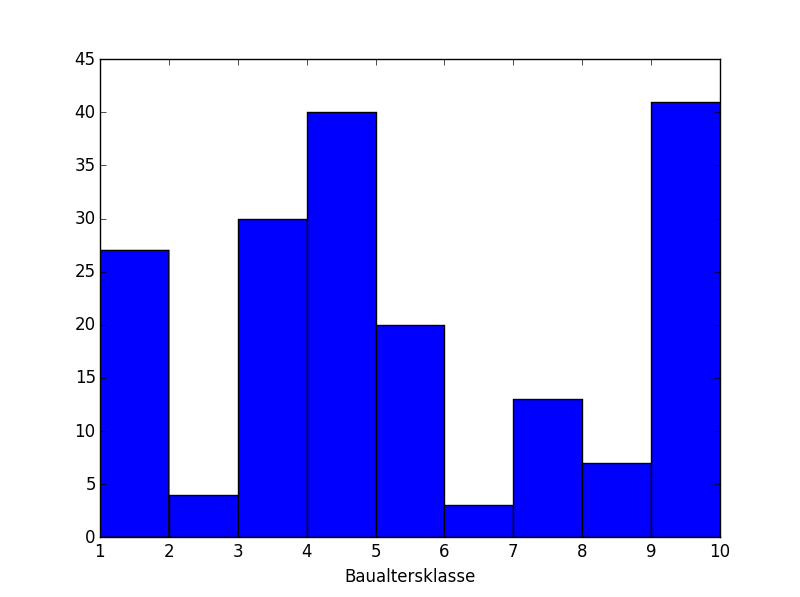
\includegraphics[width=0.60\textwidth]{Pictures/BAK.png}
	\caption{Baujahre der Gebäude}
	\label{fig:Baujahre der Gebäude}
\end{figure}
\\

Wird nun der Heizenergieverbrauchskennwert absteigend sortiert, ergibt sich eine Übersicht auf die größten Verbraucher von Heizenergie, die in Anbetracht von Baujahr und unter Einbeziehung des Vorhandenseins von Büro- und Laborflächen repräsentativ für den Gebäudebestand der RWTH stehen.  \\



\section{Gebäudesteckbrief}
\label{sec:Gebäudesteckbrief} 
Nach der Anwendung der Kriterien auf den vorliegenden Gebäudestand der Hochschule ergibt sich eine Vorauswahl von Gebäuden. \\
Weitere Gebäude mit einer Nettogrundfläche kleiner als 200m² werden aufgrund ihrer verhältnismäßig geringen Fläche aus der Betrachtung entfernt. Auffällig erscheint die Präsenz von Gebäuden der Kategorie Institutsgebäude V, welche in der gefilterten Verteilung drei der ersten fünf Gebäuden ausmacht. \\
Einen Aspekt zur Entscheidungsfindung stellt die Bereitschaft des ansässigen Institutes der Organischen Chemie dar. Die Projektleiter des Gesamtprojekts sind nach dessen Bekanntmachung kontaktiert worden, um das Interesse des Instituts Teil dieses Projektes zu werden zu bekunden. Da das Institut in zwei aneinander angrenzenden Bauten untergebracht ist, werden im Folgenden beide Gebäude betrachtet. Der sogenannte OC Turm befindet sich nach Anwendung der Kriterien der Gebäudeauswahl lediglich aufgrund einer Bürofläche von 4,86\% nicht in der zuvor betrachteten engeren Auswahl. Der Vollständigkeit halber wird das Gebäude 2031 als Anbau des Gebäudes 2030 mit einbezogen. 
\\
Aufgrund der Nutzung des Gebäudes durch ein Institut aus dem Fachbereich Chemie, ist mit einer vergleichsweise umfangreichen Anlagentechnik zu rechnen. Durch die Nutzung von Chemikalien sind in den Laborbereichen Lüftungsanlagen notwendig, wohingegen in  Büroräumen häufig manuell gelüftet wird. 
Unter Einbeziehung der Flächendaten der vorliegenden Gebäude ist die getroffene Gebäudeauswahl sehr vorteilhaft, da die Größe beider Gebäude den Aufwand rechtfertigt. \\
\\
Das Gebäude 2030 wurde im Jahr 1954 gebaut und ist somit der Baualtersklasse III zuzuordnen. Es wird vom Institut Organische Chemie genutzt und weist dadurch eine Vielzahl verschiedener Nutzungsflächen auf. Durch die Nutzung durch ein Institut aus dem Fachbereich Chemie ist das Gebäude den Institutsbauten V zuzuordnen. Die Nutzungsgesamtfläche beträgt 3960 m² und verteilt sich auf insgesamt 4 Stockwerke, welche Bibliotheks-, Büro-, Labor-, Lager- und Werkstattsflächen beinhalten. Der jährliche Verbrauch in MWh liegt in den Jahren 2011 bis 2014 zwischen 1019 und 765, bezogen auf Fläche ergeben sich Werte zwischen 340 und 268 kWh/m²NGF. Obwohl die Heizenergieverbrauchswerte innerhalb des letzten Jahres erheblich reduziert wurden, liegt der flächenspezifische Verbrauchskennwert im Jahr 2014 (268kWh/m²NGF)bei einem hohen Wert. Legt man der Analyse die Daten aus dem Jahr 2013 zugrunde, ist das betrachtete Gebäude bezüglich des Heizenergieverbrauchskennwerts auf Rang 4, in den Daten aus den Energieberichten von 2012 und 2013 sogar auf Rang 3. \\
\\
Das Gebäude 2031 ist ein Anbau an das zuvor beschriebene Gebäudes 2030 und dient dem Institut der Organischen Chemie als Erweiterung. Es wurde im Jahr 1969 an den Mitteltrakt angebaut und entspricht der Baualtersklasse V. Ebenso wie im Mitteltrakt sind verschiedene Nutzungsflächen vorhanden. Diese Flächenarten erstrecken sich über eine Fläche von 4079 m². Der Verbrauch in MWh liegt für den Zeitraum 2009 bis 2014 vor und unterliegt Schwankungen zwischen 745 und 1246. Auch bei diesem Gebäude ist für den letzten Datenwert aus dem Jahr 2014 der geringste Heizenergieverbrauch zuzuordnen. Der flächenspezifische Kennwert des Jahres 2014 liegt bei 254 kWh/m2NGF. 
Die Bauten liegen am Landoltweg 1 in Aachen und gehören zum Campus Hörn der RWTH. Beide Gebäude sind auf Grundlage des Bauwerkzuordnungskatalogs der Gruppe Institutsgebäude V zugeteilt. Diese entspricht dem Fachbereich Biologie und Chemie. 
Die Unterschiede der Heizenergiekennwerte bezogen auf den Jahresenergieverbrauch in MWh/a kommen durch die Witterungsbereinigung der Kennwerte zustande.

\section{Anlagentechnik}
\label{sec:Anlagentechnik}
 
Hauptaugenmerk bei der Betrachtung der Energieeffizienz der ausgewählten Gebäude liegt auf der Anlagentechnik, die in diesem Abschnitt detailliert beschrieben wird. Die Betrachtung der Bauphysik geschah bereits im Rahmen eines Projektes des Instituts E3d der RWTH anhand der Erstellung eines Energieausweises. Entgegen dieser statischen Betrachtung der Gebäude beschäftigt sich diese Arbeit mit der dynamischen Abbildung der Anlagentechnik.\\
\\
Pro Forma werden zwei unterschiedliche Gebäude betrachtet, allerdings erfolgt die Trennung zwischen Gebäude 2030 und 2031  lediglich durch Türen in jedem Geschoss. Beide Gebäude sind mit einem Technikraum im Dachgeschoss ausgestattet. Die Heizungsanlage des Gebäudes 2030 befindet sich im Kellergeschoss des ebenfalls direkt angrenzenden Gebäudes 2020. Die Heizung des Gebäudes 2031 befindet sich im Untergeschoss desselben Gebäudes.\\
\\
Heizung 2030\\
Die Gebäude sind an das Fernwärmenetz der STAWAG Aachen angeschlossen. Die Fernwärme tritt in Form von heißen Wasser im Untergeschoss des Nachbargebäudes 2020 mit einer Temperatur von 100°C ein. Die Versorgung des Gebäudes wird durch eine Ersatzleitung gewährleistet, die im Fall des Ausfalls der eigentlichen Leitung die Versorgung übernimmt. Im Heizungskeller wird die Wärmeenergie der Fernwärmeleitung durch einen Wärmetauscher in das Heizsystems des Gebäude 2030 übertragen. Durch diesen Wärmetauscher tritt ein erster Temperaturverlust auf. Im Kellerbereich wird dann das im Wärmetauscher erhitzte Wasser durch Heizkreispumpen der Statischen Heizung der Nord- sowie der Südseite des Gebäudes zugeführt, sowie der Statischen Heizung in der Bibliothek. Eine weitere Leitung wird den Lüftungsanlagen im Dachgeschoss zugeführt. Auch die Warmwasserbereitung wird durch die Fernwärme energetisch versorgt und auf die Nutzungsbereiche verteilt. \\
\\
Lüftungsanlagen 2030\\
Das Gebäude 2030 verfügt über zwei zentrale Lüftungsanlagen, die im 3. Obergeschoss des Gebäudes angesiedelt sind. Diese Anlagen übernehmen die Belüftung durch Zuluft sowie die Abführung der gebrauchten Abluft im Laborbereich. Die Versorgung der Bibliothek sowie des Seminarraum erfolgt durch die Zusammenführung von zwei Teilsträngen der Anlagen. Die beiden Hauptanlagen, im weiteren als Anlage 1 und Anlage 2 bezeichnet, sind wie folgt aufgebaut.\\
Die Außenluft wird mit der entsprechenden Außenlufttemperatur angesaugt. Zunächst wird sie mithilfe eines auf Druck basierenden Filters gereinigt. Abhängig von der Temperatur wird diese nach einer Volumenregelung entweder durch ein Wärmerückgewinnungsaggregat geleitet oder an diesem vorbeigeführt. Mithilfe von Glasröhren findet ein Austausch von Energie statt, der die Rückgewinnung der Wärme aus einem anderen Volumenstrom beinhaltet. Diesen zweiten Volumenstrom bildet die Abluft, die im Fall von Anlage 1 und 2 aus den Laboren des Gebäudes herausgeführt wird, und die Wärmeenergie aufgrund des Temperaturunterschiedes an die Außenluft abgibt. Daraufhin wird die Abluft aus dem Gebäude geleitet. \\
Nachdem die Außenluft wie beschrieben behandelt und erwärmt wurde, folgt die Abtrennung eines Luftstroms, der der Bibliothek und dem Seminarraum zugeführt wird und im nächsten Absatz genauer beschrieben wird. Die übrige Zuluft wird durch die Fernwärme, die im Untergeschoss des Gebäudes in das Netz eingespeist wird, erneut erwärmt. Es folgt ein weiterer Filter. Die Zuluft gelangt gemeinsam mit der Zuluft aus Anlage 2 in eine Zuluftkammer. Von dort aus wird diese in die verschiedenen Geschosse des Gebäudes weitergeleitet. Anlage 1 und 2 sind jeweils für einen Zuluftstrom von 64.000m³/h und eine Abluftvolumenstrom von 51.000m³/h ausgelegt.\\
\\
Die Lüftungsanlage die der Belüftung des Seminarraums sowie der Bibliothek dient, teilt sich in zwei seperate Stränge. Die für die Bibliothek abgezweigte Luft, die sich wie zuvor beschrieben aus dem abgeführten Luftstrom von Anlage 1 und Anlage 2 zusammensetzt, wird nochmals durch einen Filter geleitet. Es folgt ein Lufterwärmer, der die aus der Fernwärme übertragene Wärmeenergie für die Konditionierung der Lufttemperatur bereitstellt. Um die für Bibliotheken angemessenen Luftbedingungen zu erreichen, ist für den Bedarf ein Luftkühler sowie ein Entfeuchter nachgeschaltet. Die auf diese Art konditionierte Zuluft wird in die Bibliothek geleitet. Der Abluftvolumenstrom wird wie die Abluftströme aus Anlage 1 und 2 der Abluftsammelkammer im Technikraum zugeführt. 
Die Zuluft des Seminarraums durchströmt einen Filter sowie einen Lufterwärmer, der mit Energie aus dem Fernwärmenetz versorgt ist. Die so konditionierte Zuluft wird in den Seminarraum geleitet.  Wie auch die Abluft der Bibliothek wird die des Seminarraums der Abluftsammelkammer im Technikraum des 3. Obergeschosses zugeführt.\\
\\
Heizung 2031\\
Der Aufbau der Heizungsanalage des OC Turms entspricht dem Aufbau der Heizung im OC Mitteltrakt. Die Fernwärmeenergie wird mithilfe eines Wärmetauschers in das System eingebracht. Die Statische Heizung der Bibliothek ist im Gebäude 2031 nicht vorhanden, ebenso wenig wie eine Warmwasseraufbereitung. Die Statischen Heizungen auf der Nord- sowie der Südseite werden durch eine Heizkreispumpe versorgt. Ein weiterer Wärmestrom wird analog zu Gebäude 2030 den Lüftungsanlagen im Technikraum zugeführt.\\
\\
Lüftungsanlage 2031\\
Die Lüftungstechnik des Gebäudes 2031 wird durch einen Technikraum im 7. Obergeschoss gesteuert.  Es existieren zwei Lüftungsanlagen, Lüftungsanlage Nord und Lüftungsanlage Süd, die jeweils das gleiche Fließschema aufweisen.
Die Außenluft wird angesaugt, durchläuft einen Filter sowie einen Luftkühler, der durch Freie Kühlung betrieben wird. Daraufhin wird die Außenluft in einen Plattenwärmerückgewinner geführt. Die im Kreuzstrom zur Außenluft eintretende Abluft, erwärmt die kältere Außenluft. Zudem ist eine Spüleinrichtung unmittelbar nach dem Wärmerückgewinnungsaggregat installiert. Durch den Einsatz von zwei weiteren Lufterwärmern, in Form von einem Warmwasservolumenstrom der Kompressionskältemaschine und der durch Fernwärme gespeisten Heizung, wird der Luft weitere Wärmeenergie zugeführt. Mithilfe eines Filters wird die Zuluft erneut gereinigt, bevor sie in die von der Lüftungsanlage versorgten Räume im Untergeschoss bis zum 6. Obergeschoss strömt.\\
Durch die außergewöhnliche Abluftzusammensetzung, die durch die Verwendung verschiedener Chemikalien und deren Reaktionen zustande kommen, sind verschiedene Schächte zum Abführen der Laborluft notwendig. Hierbei sind die drei Kategorien Brennbare Chemikalien, Entsorgungslager und Abfüllraum von Bedeutung. Die unterschiedlichen Fraktionen müssen speziell gereinigt oder anderweitig entsorgt werden, da die Schadstoffe nicht als reine Abluft aus dem Gebäude geleitet werden können. \\
\\
Kälteerzeugung 2031 \\
Kälte entsteht im Fall einer Kompressionskältemaschine durch die Umwandlung von bestehender Wärme in negative Wärme. Die Kälteerzeugung im Gebäude 2031 basiert auf zwei seperaten Kreisläufen mit einer Leistung von jeweils 90kW. Die Kreisläufe bestehen aus 2 Kondensatoren sowie einem Verdampfer. Für den Betrieb der Kompressionskältemaschine ist das Ansaugen von Außenluft erforderlich. Diese durchströmt zunächst einen Filter, bevor sie der Kühlung von jeweils einem Kondensatoren der Kreisläufe im Kälteerzeugungsprozess dient. Im Folgenden wird die nun erwärmte Außenluft als Abluft aus dem Gebäude geleitet.\\

Die beiden anderen Kondensatoren sind mittels einer Wasserleitung an die Lüftungsanlagen 1 und 2 angeschlossen. Hierbei wird durch die Kondensatoren der Kältemaschine der Vorlauf erwärmt, welcher die Wärmeenergie dem Luftvolumenstrom zuführt, der zuvor die Wärmerückgewinnungsanlage durchlaufen ist. Das Wasser, welches nach der Erwärmung des Luftvolumenstroms zurück zur Kältemaschine geführt wird, wird wiederum zum Kondensator zurückgeführt. Hier wird die Wärmeenergie, die dem Medium der Kompressionskältemaschine entnommen wird, erneut dem Vorlauf zugeführt. 

Durch die sogenannte Freie Kühlung wird mithilfe der Temperatur der Außenluft ein Wasservolumenstrom gekühlt. Die Kältemaschine, die Freie Kühlung und der Kühlwasserkreislauf sind durch zwei Wärmetauscher miteinander verbunden. Der eine Wärmetauscher verbindet die Freie Kühlung mit dem Kühlwasserrücklauf aus dem Verteilernetz, der zweite Wärmetauscher übergibt die Wärme der Kältemaschine an den Kühlwasservorlauf. Eine Wasserleitung verbindet zudem beide Wärmetauscher miteinander. \\ Das über die Freie Kühlung gekühlte Wasser übergibt die Kälte durch beide Wärmetauscher an einen Volumenstrom, der zunächst einem Kaltwasserspeicher zugeführt wird. Vom Kaltwasserspeicher wird das Wasser durch die Verdampfer der Kompressionskältemaschine gekühlt. Dies geschieht durch das Verdampfen des Mediums der Kompressionskältemaschine, wodurch dem Kaltwasserstrom Wärmeenergie entzogen wird. Das durch die Aufwendung der Verdampfungswärme gekühlte Wasser wird bei mangelndem Bedarf unmittelbar einem Kaltwasserspeicher zugeführt, der wiederum den Rücklauf zur Kältemaschine darstellt. Danach übergibt das Wasser die negative Wärmeenergie in einem Wärmeübertrager an das Wasser, welches das Verteilernetz durchfließt. Über das Verteilernetz werden insgesamt drei Deckenumluftkühler sowie zwei Kühldecken mit Kälte versorgt. Das aus diesen Räumen zurückgeführte Wasser wird mittels zwei Dosieranlagen konditioniert und danach einem Kühlwassersammelbehälter zugeführt. Aus diesem Behälter gelangt es wieder zurück zum Wärmetauscher, der das Wasser mit negativer Wärmeenergie aus der freien Kühlung versorgt. 


\begin{equation}
\dot{Q}=\dot{p}\cdot c_p \cdot \Delta \vartheta
\end{equation}




